\section{Festigkeitslehre (Elastizitätslehre)}
Reale Körper sind deformierbar (reversibel und/oder irreversibel). Festigkeit hängt vom Material und Form ab. \\
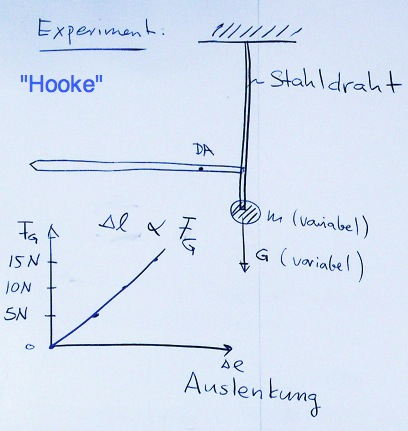
\includegraphics{Bild40}

\subsection{Materialverhalten}
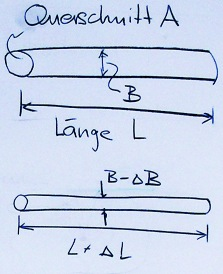
\includegraphics{Bild41} \\
\begin{def*}[ note = Dehnung , index = Dehnung ]
	\begin{gather*}
		\epsilon = \frac{\Delta L}{L} \\
		[ \epsilon ] = 1
	\end{gather*}
\end{def*}
\begin{def*}[ note = Querkontraktion , index = Querkontraktion ]
	\[ \beta = \frac{\Delta B}{B} \]
\end{def*}
\begin{def*}[ note = Normalspannung , index = Normalspannung ]
	\begin{gather*}
		\sigma = \frac{F_N}{A} \\
		[ \sigma ] = \si{\pascal}
	\end{gather*}
	Zugspannung $\sigma > 0$ \\
	Druckspannung $\sigma < 0$
\end{def*}

\subsubsection{Das Spannungs-Dehnungs Diagramm}
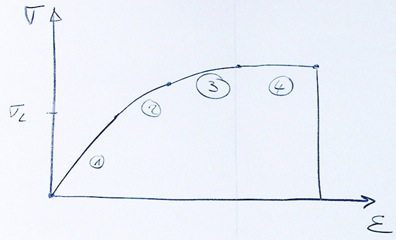
\includegraphics{Bild42} \\
\begin{enumerate}
	\item linearer Bereich $\sigma = E \epsilon$\footnote{$E$ Elastizitätsmodul, z.B. Stahl 200 GPa , Nanotubes 1TPa}
	\item nichtlinearer Bereich
	\item plastischer Bereich
	\item Fliessen
	\item Bruch
\end{enumerate}

\begin{rep*}
	\begin{itemize}
		\item Kraftstoss $\vec{F} \cdot \Delta t = \Delta \vec{p}$
		\item Derhmoment $\vec{M_o} = \vec{r} \times \vec{F}$ \\
			(Folien) \\
			gerichtete Grösse mit Drehsinn \\
			rechte Hand Regel \\
			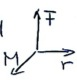
\includegraphics{Bild43}
		\item Schwerpunkt $\vec{r_{SP}} = \frac{\sum m_i \vec{r_i}}{\sum m_i}$
	\end{itemize}
	Festigkeitslehre \\
	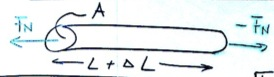
\includegraphics{Bild44} \\
	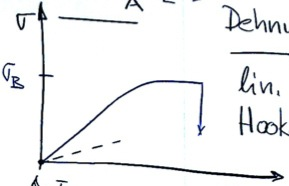
\includegraphics{Bild45}
	\begin{bsp*}
		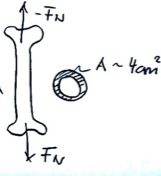
\includegraphics{Bild46}
		\[
			\sigma_{B \text{ Knochen}} = \SI{85}{\mega\pascal} \\
			\implies F_{N \text{ max}} = \sigma_B \cdot A = \SI{34}{\kilo\newton}
		\]
	\end{bsp*}
	Spannungs-Dehnungsdiagramm \\
	lin. Bereich Hooke'sches Gesetz:
	\[
		\sigma = \underbrace{E}_{\text{Elastizitätsmodul}} \cdot \epsilon \\
		\epsilon = \frac{\Delta L}{L} \quad []
	\]
\end{rep*}

\subsection{Scherung}
Demo: Schaumgummiquader \\
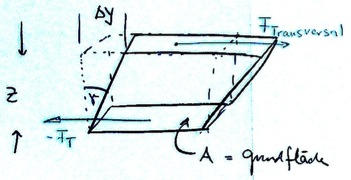
\includegraphics{Bild47} \\
Scherwinkel
\[ \gamma = \frac{\Delta y}{z} \]
\begin{def*}[ note = Schubspannung , index = Schubspannung ]
	\[
		\tau = \frac{F_T}{A} \\
		[ \tau ] = \si{\pascal}
	\]
	für den linearen Bereich (Hooke) gilt:
	\[ \tau = \underbrace{G}_{\text{Schubmodul } [ \si{\pascal} ]} \cdot \gamma \]
\end{def*}

\subsection{Spannungszustand}
Dehnung, Staucherung \\
Scherung, Biegung \\
Torsion \\
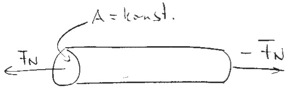
\includegraphics{Bild48} \\
Spannungsfelder
\[
	\sigma( x , y , z ) = \sigma(\vec{r}) = \frac{F_N}{A} = \text{ konst.} \\
	\tau(\vec{r}) = 0 \quad (\text{keine Scherung})
\]
Die Spannung in einem Körper lässt sich für jeden Punkt bestimmen.

\subsection{Die Biegebelastung eines Balkens}
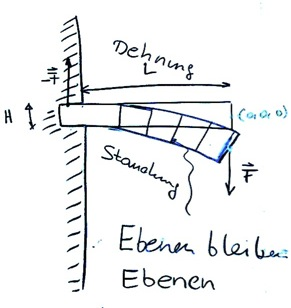
\includegraphics{Bild49} \\
Querschnitt $A = H \cdot B$ \\
Biegung:
\begin{itemize}
	\item $\sigma$ Normalspannung
	\item $\tau$ Schubspannungen
\end{itemize}
Problem: Bestimmung von $\sigma(\vec{r}) ; \tau(\vec{r})$ unter Berücksichtigung des Gleichgewichts

\subsubsection{Wahl des Koordinatensystems}
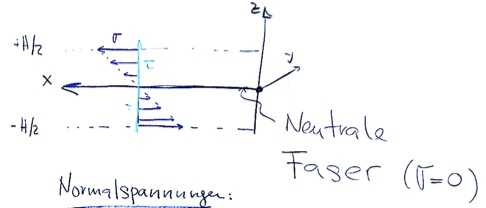
\includegraphics{Bild50} \\
Normalspannungen:
\[ \sigma( x , y , z ) = \alpha(x) \cdot z \]
prop. zur Dehnung. \\
Annahme: Gewichts des Balken $\ll F$ \\
Kräfte Gleichgewicht: \\
$z$-Komonente
\[ - F + A \cdot \tau(x) = 0 \implies \tau(x) = \frac{F}{A} = \text{ konst.} \]
$x$-Komponente:
\[
	\int_A \sigma( x , y , z ) \dd A = 0 \\
	\implies \int_{-\frac{H}{2}}^{+\frac{H}{2}} \alpha(x) \cdot z \cdot B \cdot \dd z = 0 \\
	\implies \alpha(x) \cdot B \underbrace{\int_{-\frac{H}{2}}^{+\frac{H}{2}} z \cdot \dd z}_{\text{muss $0$ sein}} = 0 \\
	\implies \text{ neutrale Faser liegt in der Mitte}
\]

\subsection{Drehmomentgleichgewicht}
\[
	\abs{M_\curvearrowright} = F \cdot x \\
	\abs{M_\curvearrowleft} = \int_A z \cdot \sigma( x , y , z ) \cdot \dd A \\
	\text{Gleichgewicht: } \abs{M_\curvearrowright} = \abs{M_\curvearrowleft} \\
	F \cdot x = \int_A z \cdot \alpha(x) \cdot z \cdot \dd A = \alpha(x) \cdot \underbrace{\overbrace{\int_A z^2 \dd A}^{\text{geometrischer Faktor}}}_{\text{Flächenträgheitsmoment } I_z} \\
	\implies \alpha( x , z ) = \alpha( x ) \cdot z = \frac{x \cdot z}{I_z} \cdot F
\]
Diskussion:
\begin{itemize}
	\item Neutrale Faser leigt bei $z=0$
	\item wo bricht der Balken bei $( L , y , \frac{H}{2} )$
	\item $I_z = \frac{1}{12} BH^3$ \\
		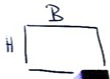
\includegraphics{Bild51}
\end{itemize}
\begin{rep*}[ note = Verteilung von Spannungen in festen Körper ]
	\begin{bsp*}[ note = Biegebelastung von Balken ]
		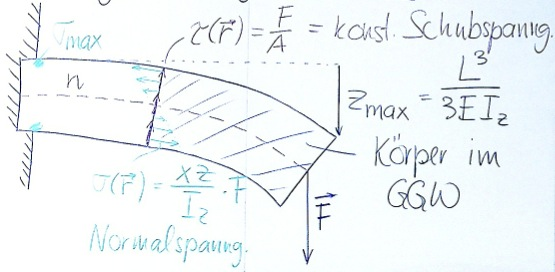
\includegraphics{Bild52} \\
		Koordinatensystem \\
		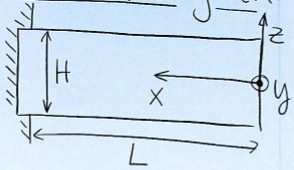
\includegraphics{Bild53} \\
		Querschnitt $A$ \\
		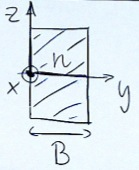
\includegraphics{Bild54}
		\[ I_z = \frac{1}{12} BH^3 \]
		Flächenträgheitsmoment $I_z$
		\[ \text{allg.:} \quad I_z = \int_A {\underbrace{z}_{\text{Abstand von $n$}}}^2 \dd z \]
	\end{bsp*}
\end{rep*}
